\documentclass[11pt,a4paper]{article}
\usepackage[margin=0.75in]{geometry}
\usepackage{amsmath,amssymb,mathtools}
\usepackage{array,booktabs,longtable,multicol}
\usepackage{tikz}
\usetikzlibrary{arrows.meta,calc,patterns,positioning}
\usepackage[most]{tcolorbox}
\usepackage{enumitem}
\usepackage{fancyhdr}
\usepackage{hyperref}
\usepackage{microtype}
\hypersetup{colorlinks=true,linkcolor=blue,urlcolor=blue}
\setlength{\parindent}{0pt}
\setlength{\parskip}{5pt}
\setlength{\headheight}{14pt}
\pagestyle{fancy}
\fancyhf{}
\lhead{BCS-012 Basic Mathematics}
\rhead{Solved Paper: December 2025}
\cfoot{\thepage}
\newcommand{\question}[1]{\vspace{0.4em}\begin{tcolorbox}[colback=gray!8,colframe=black!55,title=Question,fonttitle=\bfseries]#1\end{tcolorbox}}
\newcommand{\answer}{\textbf{Solution. }}
\newcommand{\final}[1]{\[\boxed{#1}\]}
\newcommand{\R}{\mathbb{R}}
\newcommand{\N}{\mathbb{N}}
\newcommand{\C}{\mathbb{C}}
\newcommand{\ii}{\mathrm{i}}
\begin{document}

\begin{center}
{\Large\bfseries IGNOU BCS-012: Basic Mathematics}\\[2mm]
{\large\bfseries Term-End Examination, December 2025}\\[1mm]
{\bfseries Full Solved Paper with Theory/Formula Sheet}\\[2mm]
Time: 3 Hours \quad Maximum Marks: 100
\end{center}

\begin{tcolorbox}[colback=blue!4,colframe=blue!45,title=Note]
Question No. 1 is compulsory. Attempt any three questions from the remaining questions. For practice, solutions to all questions are provided.
\end{tcolorbox}

\section*{Question 1}

\question{(a) Show that
\[
\begin{vmatrix}
-a^2 & ab & ac\\
ba & -b^2 & bc\\
ca & cb & -c^2
\end{vmatrix}=4a^2b^2c^2.
\]}
\answer
Take factors $a,b,c$ from the first, second and third rows respectively:
\[
\Delta=abc\begin{vmatrix}-a&b&c\\ a&-b&c\\ a&b&-c\end{vmatrix}.
\]
Expanding the smaller determinant along the first row,
\[
\begin{aligned}
D&=(-a)\{(-b)(-c)-bc\}-b\{a(-c)-ac\}+c\{ab-(-b)a\}\\
&=(-a)(bc-bc)-b(-2ac)+c(2ab)=0+2abc+2abc=4abc.
\end{aligned}
\]
Therefore,
\[
\Delta=abc(4abc)=4a^2b^2c^2.
\]
\final{\Delta=4a^2b^2c^2}

\question{(b) If
\[
A=\begin{pmatrix}-1&-2\\3&6\end{pmatrix},
\]
show that $A^2=5A$.}
\answer
\[
A^2=\begin{pmatrix}-1&-2\\3&6\end{pmatrix}
\begin{pmatrix}-1&-2\\3&6\end{pmatrix}
=\begin{pmatrix}1-6&2-12\\-3+18&-6+36\end{pmatrix}
=\begin{pmatrix}-5&-10\\15&30\end{pmatrix}.
\]
But
\[
5A=5\begin{pmatrix}-1&-2\\3&6\end{pmatrix}
=\begin{pmatrix}-5&-10\\15&30\end{pmatrix}.
\]
Hence $A^2=5A$.

\question{(c) Use the principle of mathematical induction to show that
\[
1+3+\cdots+(2n-1)=n^2,\quad \forall n\in\N.
\]}
\answer
Let $P(n)$ be the statement
\[
1+3+\cdots+(2n-1)=n^2.
\]
For $n=1$, LHS $=1$ and RHS $=1^2=1$. Hence $P(1)$ is true.

Assume $P(k)$ is true, that is,
\[
1+3+\cdots+(2k-1)=k^2.
\]
For $n=k+1$,
\[
\begin{aligned}
1+3+\cdots+(2k-1)+\{2(k+1)-1\}
&=k^2+(2k+1)\\
&=k^2+2k+1=(k+1)^2.
\end{aligned}
\]
Thus $P(k+1)$ is true whenever $P(k)$ is true. Hence, by induction,
\[
1+3+\cdots+(2n-1)=n^2\quad \forall n\in\N.
\]

\question{(d) If $m\ne n$ and $m$ times the $m$th term of an A.P. is equal to $n$ times the $n$th term of the A.P., show that the $(m+n)$th term is zero.}
\answer
Let the first term be $a$ and common difference be $d$. Then
\[
T_r=a+(r-1)d.
\]
Given
\[
mT_m=nT_n.
\]
So
\[
m\{a+(m-1)d\}=n\{a+(n-1)d\}.
\]
Expanding,
\[
ma+m(m-1)d=na+n(n-1)d.
\]
Bring all terms to one side:
\[
(m-n)a+\{m(m-1)-n(n-1)\}d=0.
\]
Now,
\[
m(m-1)-n(n-1)=m^2-m-n^2+n=(m-n)(m+n-1).
\]
Therefore,
\[
(m-n)\{a+(m+n-1)d\}=0.
\]
Since $m\ne n$, $m-n\ne0$. Hence
\[
a+(m+n-1)d=0.
\]
But
\[
T_{m+n}=a+(m+n-1)d.
\]
Therefore,
\[
\boxed{T_{m+n}=0}.
\]

\question{(e) If $z\in\C$ and $|z-i|=|z+i|$, show that $\operatorname{Im}(z)=0$.}
\answer
Let
\[
z=x+iy,\quad x,y\in\R.
\]
Then
\[
z-i=x+i(y-1),\qquad z+i=x+i(y+1).
\]
Using the modulus formula,
\[
|z-i|^2=x^2+(y-1)^2,
\qquad
|z+i|^2=x^2+(y+1)^2.
\]
Given $|z-i|=|z+i|$, so their squares are equal:
\[
x^2+(y-1)^2=x^2+(y+1)^2.
\]
Cancelling $x^2$,
\[
y^2-2y+1=y^2+2y+1.
\]
Therefore
\[
-2y=2y\Rightarrow 4y=0\Rightarrow y=0.
\]
Since $\operatorname{Im}(z)=y$, we get
\[
\boxed{\operatorname{Im}(z)=0}.
\]

\question{(f) Find the roots of
\[
x^3-13x^2+15x+189=0,
\]
given that one root exceeds the other by 2 and the roots are integers.}
\answer
By trial among integer factors of $189$, put $x=7$:
\[
7^3-13(7^2)+15(7)+189=343-637+105+189=0.
\]
So $x=7$ is a root and $(x-7)$ is a factor. Dividing,
\[
x^3-13x^2+15x+189=(x-7)(x^2-6x-27).
\]
Now
\[
x^2-6x-27=0
\Rightarrow
x=\frac{6\pm\sqrt{36+108}}{2}=\frac{6\pm12}{2}.
\]
Thus
\[
x=9\quad \text{or}\quad x=-3.
\]
The roots are
\[
\boxed{7,\ 9,\ -3}.
\]
Here $9$ exceeds $7$ by $2$, as required.

\question{(g) Evaluate
\[
I=\int \frac{x^3}{(x+1)^2}\,dx.
\]}
\answer
First divide $x^3$ by $(x+1)^2=x^2+2x+1$:
\[
\frac{x^3}{(x+1)^2}=x-2+\frac{3x+2}{(x+1)^2}.
\]
Write $3x+2=3(x+1)-1$. Hence
\[
\frac{3x+2}{(x+1)^2}=\frac{3}{x+1}-\frac{1}{(x+1)^2}.
\]
Therefore
\[
\begin{aligned}
I&=\int\left(x-2+\frac{3}{x+1}-\frac{1}{(x+1)^2}\right)dx\\
&=\frac{x^2}{2}-2x+3\ln|x+1|+\frac{1}{x+1}+C.
\end{aligned}
\]
\final{I=\frac{x^2}{2}-2x+3\ln|x+1|+\frac{1}{x+1}+C}

\question{(h) Show that the diagonals of a rhombus are at right angles.}
\answer
Let a rhombus have adjacent side vectors $\vec a$ and $\vec b$. Since all sides of a rhombus are equal,
\[
|\vec a|=|\vec b|.
\]
The two diagonals are represented by
\[
\vec a+\vec b
\quad\text{and}\quad
\vec a-\vec b.
\]
Their dot product is
\[
(\vec a+\vec b)\cdot(\vec a-\vec b)=\vec a\cdot\vec a-\vec b\cdot\vec b
=|\vec a|^2-|\vec b|^2=0.
\]
Since the dot product is zero, the diagonals are perpendicular.
\[
\boxed{\text{Diagonals of a rhombus are at right angles.}}
\]
\begin{center}
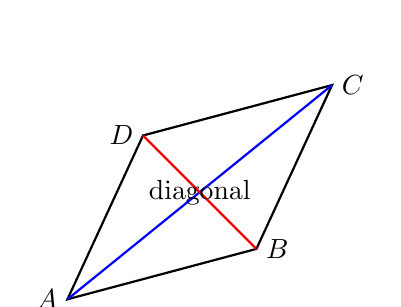
\begin{tikzpicture}[scale=0.8]
\coordinate (A) at (0,0); \coordinate (B) at (3,0.8); \coordinate (D) at (1.2,2.6); \coordinate (C) at ($(B)+(D)$);
\draw[thick] (A)--(B)--(C)--(D)--cycle;
\draw[thick,blue] (A)--(C);
\draw[thick,red] (B)--(D);
\node[left] at (A) {$A$}; \node[right] at (B) {$B$}; \node[right] at (C) {$C$}; \node[left] at (D) {$D$};
\node at (2.1,1.7) {diagonal};
\end{tikzpicture}
\end{center}

\section*{Question 2}

\question{(a) Find the 10th term of the Harmonic Progression
\[
\frac15,\frac1{11},\frac1{17},\frac1{23},\ldots
\]}
\answer
In a harmonic progression, reciprocals of the terms form an arithmetic progression. The reciprocals are
\[
5,11,17,23,\ldots
\]
This is an A.P. with first term $5$ and common difference $6$. The 10th term of this A.P. is
\[
A_{10}=5+(10-1)6=5+54=59.
\]
Therefore the 10th term of the given H.P. is
\[
\boxed{\frac1{59}}.
\]

\question{(b) If $x=a+b$, $y=a\omega+b\omega^2$ and $z=a\omega^2+b\omega$, show that $xyz=a^3+b^3$, where $\omega\ne1$ is a cube root of unity.}
\answer
For cube roots of unity,
\[
1+\omega+\omega^2=0,\qquad \omega^3=1.
\]
Now
\[
xyz=(a+b)(a\omega+b\omega^2)(a\omega^2+b\omega).
\]
First multiply the last two factors:
\[
\begin{aligned}
(a\omega+b\omega^2)(a\omega^2+b\omega)
&=a^2\omega^3+ab\omega^2+ab\omega^4+b^2\omega^3\\
&=a^2+ab(\omega^2+\omega)+b^2\\
&=a^2-ab+b^2.
\end{aligned}
\]
Therefore,
\[
xyz=(a+b)(a^2-ab+b^2)=a^3+b^3.
\]
Hence proved.

\question{(c) Find the direction cosines of the line joining $(0,1,-1)$ and $(3,2,1)$.}
\answer
Direction ratios of the line are obtained by subtracting coordinates:
\[
(3-0,\ 2-1,\ 1-(-1))=(3,1,2).
\]
The magnitude is
\[
\sqrt{3^2+1^2+2^2}=\sqrt{14}.
\]
Therefore the direction cosines are
\[
\boxed{\left(\frac3{\sqrt{14}},\frac1{\sqrt{14}},\frac2{\sqrt{14}}\right)}.
\]

\question{(d) If
\[
y=\frac{e^x+e^{-x}}{e^x-e^{-x}},
\]
find $\dfrac{dy}{dx}$.}
\answer
Let
\[
u=e^x+e^{-x},\qquad v=e^x-e^{-x}.
\]
Then
\[
u'=e^x-e^{-x}=v,
\qquad
v'=e^x+e^{-x}=u.
\]
Using the quotient rule,
\[
\frac{dy}{dx}=\frac{v u'-u v'}{v^2}=\frac{v^2-u^2}{v^2}.
\]
Now
\[
v^2-u^2=(v-u)(v+u)=(-2e^{-x})(2e^x)=-4.
\]
Hence
\[
\boxed{\frac{dy}{dx}=\frac{-4}{(e^x-e^{-x})^2}}.
\]

\section*{Question 3}

\question{(a) If
\[
y=\ln\left[e^x\left(\frac{x-2}{x+2}\right)^{3/4}\right],
\]
show that
\[
\frac{dy}{dx}=\frac{x^2-1}{x^2-4}.
\]}
\answer
Using logarithmic laws,
\[
y=x+\frac34\ln\left(\frac{x-2}{x+2}\right)
=x+\frac34\{\ln(x-2)-\ln(x+2)\}.
\]
Differentiating,
\[
\frac{dy}{dx}=1+\frac34\left(\frac1{x-2}-\frac1{x+2}\right).
\]
Now
\[
\frac1{x-2}-\frac1{x+2}=\frac{(x+2)-(x-2)}{(x-2)(x+2)}=\frac4{x^2-4}.
\]
Therefore
\[
\frac{dy}{dx}=1+\frac34\cdot\frac4{x^2-4}=1+\frac3{x^2-4}
=\frac{x^2-4+3}{x^2-4}=\frac{x^2-1}{x^2-4}.
\]
Hence proved.

\question{(b) Find the intervals in which
\[
f(x)=3x^{5/2}-5x^{3/2},\quad x>0,
\]
is increasing and decreasing.}
\answer
Differentiate:
\[
f'(x)=3\cdot\frac52x^{3/2}-5\cdot\frac32x^{1/2}
=\frac{15}{2}x^{1/2}(x-1).
\]
Since $x>0$, $x^{1/2}>0$. Therefore the sign of $f'(x)$ depends on $(x-1)$.
\[
\begin{array}{c|c|c}
\text{Interval} & f'(x) & \text{Nature}\\\hline
(0,1)& - & \text{decreasing}\\
(1,\infty)& + & \text{increasing}
\end{array}
\]
Hence
\[
\boxed{\text{decreasing on }(0,1),\quad \text{increasing on }(1,\infty).}
\]

\question{(c) Evaluate
\[
\int \frac{3^x+2^x}{6^x}\,dx.
\]}
\answer
Since $6^x=(2\cdot3)^x=2^x3^x$,
\[
\frac{3^x+2^x}{6^x}=\frac{3^x}{2^x3^x}+\frac{2^x}{2^x3^x}=2^{-x}+3^{-x}.
\]
Therefore
\[
\begin{aligned}
\int \frac{3^x+2^x}{6^x}\,dx
&=\int (2^{-x}+3^{-x})dx\\
&=-\frac{2^{-x}}{\ln 2}-\frac{3^{-x}}{\ln 3}+C.
\end{aligned}
\]
\final{-\frac{2^{-x}}{\ln 2}-\frac{3^{-x}}{\ln 3}+C}

\question{(d) If
\[
\vec a=4\hat i+\hat j+3\hat k,
\qquad
\vec b=-2\hat i+\hat j-2\hat k,
\]
find a unit vector perpendicular to both $\vec a$ and $\vec b$.}
\answer
A vector perpendicular to both $\vec a$ and $\vec b$ is $\vec a\times\vec b$:
\[
\vec a\times\vec b=
\begin{vmatrix}
\hat i&\hat j&\hat k\\
4&1&3\\
-2&1&-2
\end{vmatrix}.
\]
Thus
\[
\vec a\times\vec b=\hat i(1\cdot(-2)-3\cdot1)-\hat j(4\cdot(-2)-3\cdot(-2))+\hat k(4\cdot1-1\cdot(-2)).
\]
So
\[
\vec a\times\vec b=-5\hat i+2\hat j+6\hat k.
\]
Its magnitude is
\[
\sqrt{(-5)^2+2^2+6^2}=\sqrt{65}.
\]
Therefore a required unit vector is
\[
\boxed{\frac{-5\hat i+2\hat j+6\hat k}{\sqrt{65}}}.
\]
The opposite vector is also correct.

\section*{Question 4}

\question{(a) If $x\in\R$, solve the inequality
\[
\frac9{x-3}<5.
\]}
\answer
Bring all terms to one side:
\[
\frac9{x-3}-5<0.
\]
Taking common denominator,
\[
\frac{9-5(x-3)}{x-3}<0
\Rightarrow
\frac{24-5x}{x-3}<0.
\]
Critical values are
\[
x=3\quad \text{and}\quad x=\frac{24}{5}.
\]
Check signs on intervals:
\[
\begin{array}{c|c}
\text{Interval} & \dfrac{24-5x}{x-3}\\\hline
(-\infty,3) & - \\
(3,24/5) & + \\
(24/5,\infty) & -
\end{array}
\]
Hence the solution set is
\[
\boxed{(-\infty,3)\cup\left(\frac{24}{5},\infty\right)}.
\]
\begin{center}
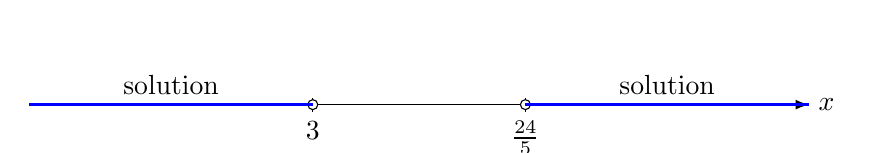
\begin{tikzpicture}[scale=0.9]
\draw[-Latex] (-4,0)--(7,0) node[right] {$x$};
\foreach \x/\lab in {0/3,3/\frac{24}{5}}{
  \draw (\x,0.1)--(\x,-0.1) node[below] {$\lab$};
  \draw[fill=white] (\x,0) circle (2pt);
}
\draw[very thick,blue] (-4,0)--(0,0);
\draw[very thick,blue] (3,0)--(7,0);
\node[above] at (-2,0) {solution};
\node[above] at (5,0) {solution};
\end{tikzpicture}
\end{center}

\question{(b) If $a,b,x,y\in\R$, $a\ne0$, $b\ne0$ and
\[
(a-ib)(x+iy)=(a^2+b^2)i,
\]
find $x$ and $y$.}
\answer
Expand the left side:
\[
(a-ib)(x+iy)=ax+iay-ibx+by=(ax+by)+i(ay-bx).
\]
Equating real and imaginary parts with $0+i(a^2+b^2)$, we get
\[
ax+by=0,
\qquad
ay-bx=a^2+b^2.
\]
From $ax+by=0$,
\[
by=-ax.
\]
The values $x=-b$ and $y=a$ satisfy
\[
a(-b)+b(a)=0,
\]
and
\[
a(a)-b(-b)=a^2+b^2.
\]
Therefore
\[
\boxed{x=-b,\quad y=a}.
\]

\question{(c) Use Cramer's rule to solve
\[
2x-y+z=4,\qquad 3x-y=5,
\qquad 2y-z=1.
\]}
\answer
Write the system as $AX=B$:
\[
A=\begin{pmatrix}2&-1&1\\3&-1&0\\0&2&-1\end{pmatrix},
\quad
X=\begin{pmatrix}x\\y\\z\end{pmatrix},
\quad
B=\begin{pmatrix}4\\5\\1\end{pmatrix}.
\]
The determinant of $A$ is
\[
\Delta=\begin{vmatrix}2&-1&1\\3&-1&0\\0&2&-1\end{vmatrix}=1.
\]
Replacing columns by $B$ gives
\[
\Delta_x=\begin{vmatrix}4&-1&1\\5&-1&0\\1&2&-1\end{vmatrix}=2,
\]
\[
\Delta_y=\begin{vmatrix}2&4&1\\3&5&0\\0&1&-1\end{vmatrix}=1,
\]
\[
\Delta_z=\begin{vmatrix}2&-1&4\\3&-1&5\\0&2&1\end{vmatrix}=1.
\]
By Cramer's rule,
\[
x=\frac{\Delta_x}{\Delta}=2,
\quad
y=\frac{\Delta_y}{\Delta}=1,
\quad
z=\frac{\Delta_z}{\Delta}=1.
\]
\final{x=2,\ y=1,\ z=1}

\question{(d) If
\[
A=\begin{pmatrix}2&2&-4\\-4&2&-4\\2&-1&5\end{pmatrix},
\quad
B=\begin{pmatrix}1&-1&0\\2&3&4\\0&1&2\end{pmatrix},
\]
show that $AB=BA=6I_3$. Find $A^{-1}$.}
\answer
Compute $AB$:
\[
AB=\begin{pmatrix}2&2&-4\\-4&2&-4\\2&-1&5\end{pmatrix}
\begin{pmatrix}1&-1&0\\2&3&4\\0&1&2\end{pmatrix}
=\begin{pmatrix}6&0&0\\0&6&0\\0&0&6\end{pmatrix}=6I_3.
\]
Similarly,
\[
BA=\begin{pmatrix}1&-1&0\\2&3&4\\0&1&2\end{pmatrix}
\begin{pmatrix}2&2&-4\\-4&2&-4\\2&-1&5\end{pmatrix}
=\begin{pmatrix}6&0&0\\0&6&0\\0&0&6\end{pmatrix}=6I_3.
\]
Thus
\[
AB=BA=6I_3.
\]
Dividing by $6$,
\[
A\left(\frac16B\right)=I_3.
\]
Therefore
\[
A^{-1}=\frac16B.
\]
Hence
\[
\boxed{A^{-1}=\frac16\begin{pmatrix}1&-1&0\\2&3&4\\0&1&2\end{pmatrix}}.
\]

\section*{Question 5}

\question{(a) Use mathematical induction to show that
\[
1+\frac12+\frac1{2^2}+\cdots+\frac1{2^n}<2,
\quad \forall n\in\N.
\]}
\answer
Let
\[
P(n):\quad 1+\frac12+\frac1{2^2}+\cdots+\frac1{2^n}<2.
\]
For $n=1$,
\[
1+\frac12=\frac32<2,
\]
so $P(1)$ is true.

Assume $P(k)$ is true, i.e.
\[
1+\frac12+\frac1{2^2}+\cdots+\frac1{2^k}<2.
\]
For $n=k+1$,
\[
S_{k+1}=S_k+\frac1{2^{k+1}}.
\]
To get a sharper bound, use the finite G.P. sum for $S_k$:
\[
S_k=1+\frac12+\cdots+\frac1{2^k}=2-\frac1{2^k}.
\]
Thus
\[
S_{k+1}=2-\frac1{2^k}+\frac1{2^{k+1}}
=2-\frac1{2^{k+1}}<2.
\]
Therefore $P(k+1)$ is true. Hence, by mathematical induction,
\[
\boxed{1+\frac12+\frac1{2^2}+\cdots+\frac1{2^n}<2\quad \forall n\in\N.}
\]

\question{(b) Find the quadratic equation with real coefficients if one of its roots is $-2+3i$.}
\answer
For a quadratic equation with real coefficients, complex roots occur in conjugate pairs. Hence the other root is
\[
-2-3i.
\]
The required equation is
\[
(x-(-2+3i))(x-(-2-3i))=0.
\]
Thus
\[
(x+2-3i)(x+2+3i)=0.
\]
Using $(p-q)(p+q)=p^2-q^2$,
\[
(x+2)^2-(3i)^2=0.
\]
Since $i^2=-1$,
\[
(x+2)^2+9=0.
\]
Therefore
\[
x^2+4x+4+9=0.
\]
\final{x^2+4x+13=0}

\question{(c) If
\[
\vec a=-\hat i+\hat j+2\hat k,
\quad
\vec b=2\hat i-\hat j+\hat k,
\quad
\vec c=3\hat i-\hat j+2\hat k,
\]
find $(\vec a\times\vec b)\cdot\vec c$.}
\answer
First compute
\[
\vec a\times\vec b=\begin{vmatrix}
\hat i&\hat j&\hat k\\
-1&1&2\\
2&-1&1
\end{vmatrix}.
\]
Thus
\[
\vec a\times\vec b
=\hat i(1\cdot1-2(-1))-\hat j((-1)\cdot1-2\cdot2)+\hat k((-1)(-1)-1\cdot2).
\]
So
\[
\vec a\times\vec b=3\hat i+5\hat j-\hat k.
\]
Now
\[
(\vec a\times\vec b)\cdot\vec c=(3,5,-1)\cdot(3,-1,2).
\]
Therefore
\[
(\vec a\times\vec b)\cdot\vec c=9-5-2=2.
\]
\final{(\vec a\times\vec b)\cdot\vec c=2}

\question{(d) Maximize
\[
P=5x+2y
\]
subject to
\[
10x+2y\ge2100,
\quad
x+\frac12y\le600,
\quad
y\le800,
\quad
x\ge0,
\quad
y\ge0.
\]}
\answer
Simplify the first two inequalities:
\[
10x+2y\ge2100\Rightarrow 5x+y\ge1050,
\]
\[
x+\frac12y\le600\Rightarrow 2x+y\le1200.
\]
The feasible region is bounded by
\[
5x+y=1050,
\quad
2x+y=1200,
\quad
y=800,
\quad
x=0,
\quad
y=0.
\]
The relevant corner points are
\[
(50,800),\quad (200,800),\quad (600,0),\quad (210,0).
\]
Evaluate $P=5x+2y$ at these points:
\[
\begin{array}{c|c}
\text{Corner point} & P=5x+2y\\\hline
(50,800)&250+1600=1850\\
(200,800)&1000+1600=2600\\
(600,0)&3000\\
(210,0)&1050
\end{array}
\]
The maximum value is $3000$ at $(600,0)$.
\[
\boxed{P_{\max}=3000\text{ at }(x,y)=(600,0).}
\]
\begin{center}
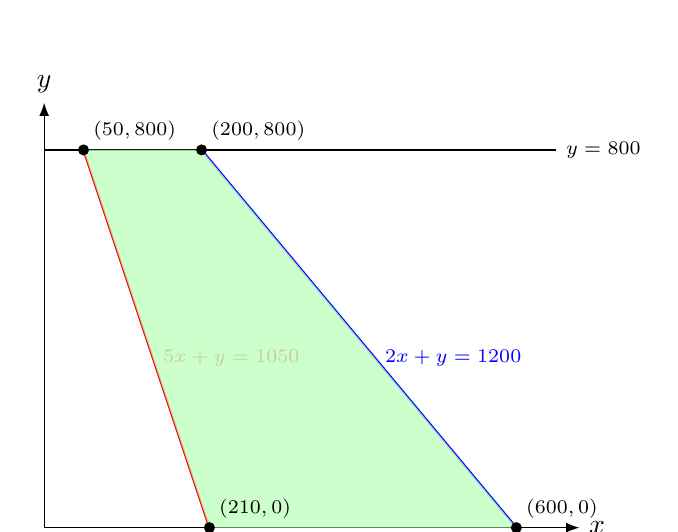
\begin{tikzpicture}[x=0.01cm,y=0.006cm]
\draw[-Latex] (0,0)--(680,0) node[right] {$x$};
\draw[-Latex] (0,0)--(0,900) node[above] {$y$};
\draw[thick,red] (50,800)--(210,0) node[pos=0.55,right] {\scriptsize $5x+y=1050$};
\draw[thick,blue] (200,800)--(600,0) node[pos=0.55,right] {\scriptsize $2x+y=1200$};
\draw[thick] (0,800)--(650,800) node[right] {\scriptsize $y=800$};
\fill[green!25,opacity=0.8] (50,800)--(200,800)--(600,0)--(210,0)--cycle;
\foreach \x/\y/\lab in {50/800/{(50,800)},200/800/{(200,800)},600/0/{(600,0)},210/0/{(210,0)}}{
  \fill (\x,\y) circle (2pt);
  \node[above right] at (\x,\y) {\scriptsize $\lab$};
}
\end{tikzpicture}
\end{center}

\newpage
\section*{Theory and Formula Sheet for This Paper}

\begin{multicols}{2}
\subsection*{Determinants and Matrices}
\begin{itemize}[leftmargin=*]
\item Row/column factors can be taken outside a determinant.
\item If $AB=BA=I$, then $B=A^{-1}$.
\item If $AB=BA=kI$, then $A^{-1}=\frac1kB$.
\item Cramer's rule: for $AX=B$, $x_i=\Delta_i/\Delta$, where $\Delta=|A|\ne0$.
\end{itemize}

\subsection*{Sequences}
\begin{itemize}[leftmargin=*]
\item A.P.: $T_n=a+(n-1)d$.
\item H.P.: reciprocals of H.P. terms form an A.P.
\item Finite G.P.: $S_n=a\dfrac{1-r^n}{1-r}$ for $r\ne1$.
\item Sum of first $n$ odd numbers: $1+3+\cdots+(2n-1)=n^2$.
\end{itemize}

\subsection*{Complex Numbers}
\begin{itemize}[leftmargin=*]
\item If $z=x+iy$, then $|z|=\sqrt{x^2+y^2}$ and $\operatorname{Im}(z)=y$.
\item For real-coefficient quadratic equations, non-real complex roots occur in conjugate pairs.
\item Cube roots of unity: $1,\omega,\omega^2$ with $1+\omega+\omega^2=0$ and $\omega^3=1$.
\end{itemize}

\subsection*{Calculus}
\begin{itemize}[leftmargin=*]
\item Quotient rule: $\left(\dfrac uv\right)'=\dfrac{vu'-uv'}{v^2}$.
\item Log rule: $\ln(ab)=\ln a+\ln b$, $\ln(a^r)=r\ln a$.
\item $\dfrac{d}{dx}a^x=a^x\ln a$.
\item $\int a^x\,dx=\dfrac{a^x}{\ln a}+C$ for $a>0$, $a\ne1$.
\item Function increasing when $f'(x)>0$ and decreasing when $f'(x)<0$.
\end{itemize}

\subsection*{Vectors and 3D Geometry}
\begin{itemize}[leftmargin=*]
\item Direction cosines of vector $(l,m,n)$ are
$\left(\dfrac{l}{\sqrt{l^2+m^2+n^2}},\dfrac{m}{\sqrt{l^2+m^2+n^2}},\dfrac{n}{\sqrt{l^2+m^2+n^2}}\right)$.
\item A vector perpendicular to both $\vec a$ and $\vec b$ is $\vec a\times\vec b$.
\item Unit vector in direction $\vec v$ is $\vec v/|\vec v|$.
\item Scalar triple product: $(\vec a\times\vec b)\cdot\vec c$.
\item Diagonals of a rhombus: if side vectors are $\vec a,\vec b$ and $|\vec a|=|\vec b|$, then $(\vec a+\vec b)\cdot(\vec a-\vec b)=0$.
\end{itemize}

\subsection*{Inequalities and LPP}
\begin{itemize}[leftmargin=*]
\item For rational inequalities, bring to one side, find critical points, and test intervals.
\item In linear programming, optimum occurs at a corner point of the feasible region.
\item Evaluate the objective function at all feasible corner points and choose maximum/minimum.
\end{itemize}
\end{multicols}

\end{document}
